\documentclass[aps,prl,reprint,superscriptaddress,nofootinbib]{revtex4-2}
\usepackage{amsmath,amssymb,bm,graphicx,booktabs}
\usepackage{xcolor}
\usepackage{tikz}
\usetikzlibrary{arrows.meta,positioning,calc,fit}
\graphicspath{{figures/}}

\newcommand{\CP}{\mathbb{CP}}
\newcommand{\ii}{\mathrm{i}}
\newcommand{\resultneeded}[1]{\textbf{\color{red!70!black}[RESULT NEEDED: #1]}}

\begin{document}
\title{Projective Outcome Geometry and Born-Like Dipoles in Unitary Many-Body Detectors}
\author{Authors withheld for review}
\affiliation{Affiliation withheld for review}
\date{August 14, 2026}

\begin{abstract}
Can measurement be another apparent arrow of time emerging from globally unitary many-body dynamics?  We formulate a precise restricted-state loophole: product inputs that a finite qubit--detector propagator maps to a definite qubit pole are the projective roots of a detector-space matrix pencil.  Unitarity further forces the two outcome-root multisets to be exact Bloch antipodes, so a regular detector of dimension $d$ produces $d$ projective roots and their labelled partners.  For Haar propagators the roots are exactly the complex spherical ensemble and have uniform one-point intensity, precluding a fixed ensemble-selected measurement axis.  In a post-cutoff many-body dataset, a clean matched-field spin ring instead develops a Born-like dipolar root-count geometry: the four-time median polar score rises from $0.192$ at $N=11$ to $0.807$ at $N=16$, while an $N=16$ full-sphere map has unit coverage and a count-weighted Born residual $0.089$.  These results establish exact boundary-compatible states and a structured-versus-Haar distinction; a physical measure selecting those states and stable detector records remain open.
\end{abstract}
\maketitle

% FIGURE 1 SOURCE: reproducible TikZ in this file; no empirical data.
\begin{figure*}[t]
\centering
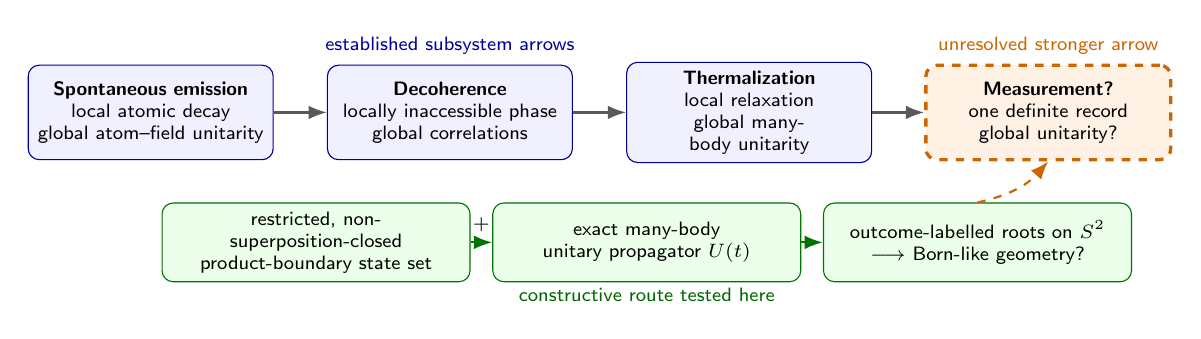
\begin{tikzpicture}[
  font=\sffamily\scriptsize,
  >=Latex,
  established/.style={draw=blue!60!black,fill=blue!6,rounded corners,align=center,
    minimum height=12mm,text width=29mm,inner sep=3pt},
  unresolved/.style={draw=orange!80!black,fill=orange!10,rounded corners,align=center,
    minimum height=12mm,text width=29mm,inner sep=3pt,dashed,very thick},
  route/.style={draw=green!45!black,fill=green!8,rounded corners,align=center,
    minimum height=10mm,text width=37mm,inner sep=3pt},
  arrow/.style={->,thick,draw=black!65}
]
\node[established] (se) at (0,0) {\textbf{Spontaneous emission}\\local atomic decay\\global atom--field unitarity};
\node[established] (dc) at (3.8,0) {\textbf{Decoherence}\\locally inaccessible phase\\global correlations};
\node[established] (th) at (7.6,0) {\textbf{Thermalization}\\local relaxation\\global many-body unitarity};
\node[unresolved] (me) at (11.4,0) {\textbf{Measurement?}\\one definite record\\global unitarity?};
\draw[arrow] (se) -- (dc);
\draw[arrow] (dc) -- (th);
\draw[arrow] (th) -- (me);
\node[route] (rs) at (2.1,-1.65) {restricted, non-superposition-closed\\product-boundary state set};
\node[route] (ud) at (6.3,-1.65) {exact many-body\\unitary propagator $U(t)$};
\node[route] (sp) at (10.5,-1.65) {outcome-labelled roots on $S^2$\\$\longrightarrow$ Born-like geometry?};
\draw[arrow,draw=green!45!black] (rs) -- node[above] {$+$} (ud);
\draw[arrow,draw=green!45!black] (ud) -- (sp);
\draw[->,dashed,thick,draw=orange!80!black] (sp.north) to[bend right=18] (me.south);
\node[blue!60!black] at (3.8,0.85) {established subsystem arrows};
\node[orange!80!black] at (11.4,0.85) {unresolved stronger arrow};
\node[green!40!black] at (6.3,-2.32) {constructive route tested here};
\end{tikzpicture}
\caption{\textbf{Quantum arrows of time.}  Spontaneous emission, decoherence, and thermalization reconcile apparently irreversible local behavior with reversible global dynamics.  Measurement asks for the stronger step from a superposition of alternatives to one global record.  This work tests a restricted-state loophole while retaining exact unitarity; the arrow itself is motivation, not a theorem.}
\label{fig:arrow}
\end{figure*}

Spontaneous emission is an elementary subsystem arrow; decoherence and thermalization show the same broad pattern, in which accessible local phase information or memory is lost while the complete state evolves unitarily~\cite{Zurek2003,Deutsch1991,Srednicki1994}.  Decoherence and quantum Darwinism explain pointer stability and the local availability of classical information~\cite{BrandaoPianiHorodecki2015,QiRanard2021,DoucetDeffner2024}; they do not, by themselves, replace a global superposition of records by one term.  Measurement is therefore the unresolved fourth arrow in Fig.~\ref{fig:arrow}.

The obstruction is linearity: if basis inputs produce distinct records, an unrestricted superposition principle makes their superposition produce a superposition of records~\cite{BassiGhirardi2000}.  We retain exact global unitarity but investigate a narrower premise---that physically realized global product states might occupy a dynamically defined set not closed under arbitrary addition.  This is a constructive loophole adjacent to special-state approaches~\cite{Schulman2012,Schulman2017}, not a derived law of nature.

\emph{Exact construction.}---Let the readout qubit be the first factor of $\mathbb C^2\otimes\mathbb C^d$ and write
\begin{equation}
 U=\begin{pmatrix}A&B\\C&D\end{pmatrix},\qquad A,B,C,D\in\mathbb C^{d\times d}.       \label{eq:block}
\end{equation}
For a homogeneous qubit coordinate $q=[\alpha:\beta]\in\CP^1$, a product input reaches pole $0$ precisely when
\begin{equation}
 (\alpha C+\beta D)\eta=0,                                                       \label{eq:pencil0}
\end{equation}
and reaches pole $1$ when $(\alpha A+\beta B)\eta=0$.  In the affine chart $z=\beta/\alpha=e^{\ii\phi}\tan(\theta/2)$ these are the pencils $C+zD$ and $A+zB$; $z=\infty$ is retained projectively.  A regular $d\times d$ pencil has exactly $d$ roots in $\CP^1$, counted with algebraic multiplicity, although roots may coincide and singular pencils require Kronecker rather than eigenvalue analysis~\cite{MolerStewart1973,Supplement}.

Unitarity supplies a stronger relation absent from root counting alone.  With the antipodal coordinate $q^\perp=[-\bar\beta:\bar\alpha]$, Jacobi complementary-minor duality gives
\begin{equation}
 \det(\alpha C+\beta D)=(-1)^d\det(U)\,
 \overline{\det(-\bar\beta A+\bar\alpha B)}.                                  \label{eq:duality}
\end{equation}
Thus the two outcome-root multisets are exact Bloch antipodes, including multiplicity.  There are $d$ projective coordinates and their labelled partners, not two unrelated $d$-clouds.  Consequently
\begin{equation}
 \rho_1(\Omega)=\rho_0(-\Omega),\quad
 a(\Omega)=\frac{\rho_0(\Omega)-\rho_0(-\Omega)}{\rho_0(\Omega)+\rho_0(-\Omega)},                 \label{eq:asymmetry}
\end{equation}
and $a(-\Omega)=-a(\Omega)$.  An ideal projective measurement is the pure dipole $a_{\rm B}(\Omega)=\hat{\bm n}\cdot\bm r(\Omega)$; the first allowed non-Born multipoles are odd $\ell\geq3$.  The total root density need not be uniform.

% FIGURE 2 SOURCE: reproducible TikZ in this file; no empirical data.
\begin{figure}[t]
\centering
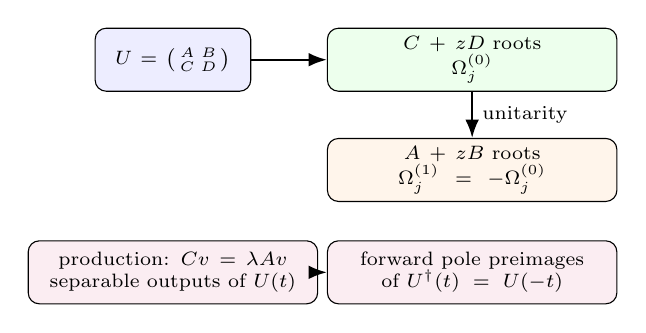
\begin{tikzpicture}[font=\scriptsize,>=Latex,
 box/.style={draw,rounded corners,align=center,inner sep=2.5pt,text width=18mm,minimum height=8mm},
 wide/.style={draw,rounded corners,align=center,inner sep=2.5pt,text width=35mm,minimum height=8mm}]
\node[box,fill=blue!7] (u) at (0,1.35) {$U=\left(\begin{smallmatrix}A&B\\C&D\end{smallmatrix}\right)$};
\node[wide,fill=green!7] (p) at (3.8,1.35) {$C+zD$ roots\\$\Omega_j^{(0)}$};
\node[wide,fill=orange!8] (a) at (3.8,-0.05) {$A+zB$ roots\\$\Omega_j^{(1)}=-\Omega_j^{(0)}$};
\draw[->,thick] (u) -- (p);
\draw[->,thick] (p) -- node[right] {unitarity} (a);
\node[wide,fill=purple!7] (prod) at (0,-1.35) {production: $Cv=\lambda Av$\\separable outputs of $U(t)$};
\node[wide,fill=purple!7] (inv) at (3.8,-1.35) {forward pole preimages\\of $U^\dagger(t)=U(-t)$};
\draw[->,thick,dashed] (prod) -- (inv);
\end{tikzpicture}
\caption{\textbf{Projective construction and numerical bridge.}  The forward pencils give exact pole-compatible inputs and unitarity fixes the second outcome coordinates antipodally.  Production data solve the related fixed-input-pole pencil; inverse evolution converts its separable outputs into forward pole preimages.}
\label{fig:construction}
\end{figure}

The special product cone is generically nonadditive: for a regular pencil with two distinct roots, the sum of compatible states has Schmidt rank two.  The full pole-preimage subspace $U^\dagger(|k\rangle\otimes\mathcal H_D)$ remains linear, however; identifying only its product intersection with physically realized states is an additional hypothesis.

\emph{Haar null model.}---For Haar $U(2d)$, the adjoint block row $(C^\dagger,D^\dagger)^T$ is a Haar Stiefel frame.  Its Ginibre representation contains a common invertible factor that cancels from Eq.~\eqref{eq:pencil0}; the roots are therefore exactly the complex spherical ensemble~\cite{Krishnapur2009,AlishahiZamani2015}.  Its one-point intensity is $d/(4\pi)$ per solid angle for every $d$.  Haar dynamics consequently has no preferred fixed axis at the ensemble one-point level: its normalized ensemble fraction $\bar\rho_0/(\bar\rho_0+\bar\rho_1)$ is $1/2$ at every point, not a fixed-axis Born dipole.  A finite cloud can have realization-dependent anisotropy; this exact ensemble statement is not a concentration bound.

\emph{Many-body evidence.}---For finite roots, the production campaigns fix the input pole and solve
\begin{equation}
 Cv=\lambda Av,\qquad U(|0\rangle\otimes v)=(|0\rangle+\lambda|1\rangle)\otimes Av. \label{eq:production}
\end{equation}
These output roots are the forward pole-$0$ preimages of $U^\dagger$.  The outcome-$1$ coordinates follow from Eq.~\eqref{eq:duality}.  For the real Hamiltonian below, forward evolution at $+t$ reflects $\phi$ relative to the displayed production convention but leaves $\theta$ and all fixed-$z$ Born diagnostics invariant.

The strongest post--July 1, 2026 dataset is a clean ring of $N$ detector spins,
\begin{align}
H={}&-h_{z0}Z_0-h_z\sum_iZ_i-J\sum_iZ_iZ_{i+1}\nonumber\\
&-J_{\pm}\sum_i(\sigma_i^+\sigma_{i+1}^-+\mathrm{H.c.})\nonumber\\
&-\frac{J_x}{\sqrt N}X_0\sum_iX_i-\frac{J_y}{\sqrt N}Y_0\sum_iY_i.              \label{eq:H}
\end{align}
with periodic detector bonds, $h_{z0}=h_z=0.1$, $J=1$, $J_\pm=J_y=0$, and collective $J_x=0.01$ in repository units ($\hbar=1$).

% NUMERICAL PROVENANCE:
% generated: 2026-08-14 post-processing of a run completed 2026-07-15T14:15:06Z
% script: prl_draft/scripts/build_figures.py
% data: work/zeus_single_pixel_atlas_scaling_2026-07-14/hz0/N16/raw/N16/hz0_+0.1000/raw_t10000.npz
% configuration: h_z0=h_z=0.1, J=1, J_pm=J_y=0, collective J_x=0.01
% system size: N=16 detector spins (17 total qubits); 65,536 finite roots
% samples: one deterministic Hamiltonian/time, t=10^4; 36x18 equal-area grid; no smoothing
% seeds: none
% commit: working tree recorded in NUMERICAL_PROVENANCE.md
\begin{figure*}[t]
\centering
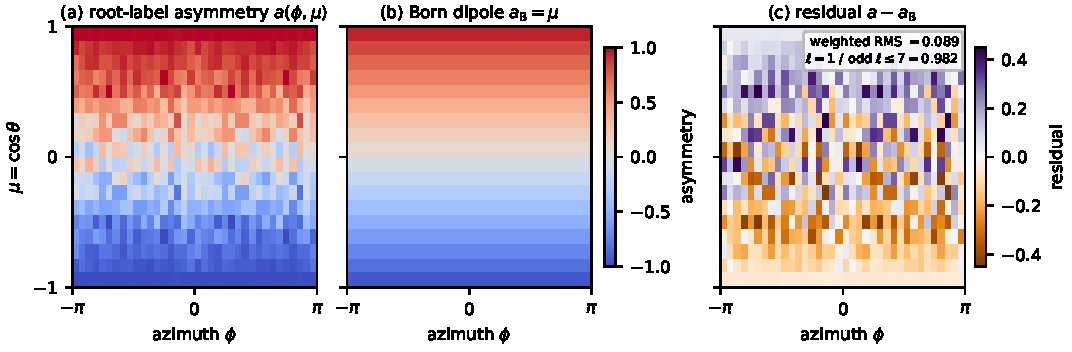
\includegraphics[width=0.98\textwidth]{full_sphere_matched.pdf}
\caption{\textbf{Full-sphere matched-ring geometry.}  At $N=16,t=10^4$, the root cloud and its exact antipodal outcome partners define the equal-area asymmetry $a(\phi,\mu)$, $\mu=\cos\theta$ (36 azimuthal by 18 polar bins, no smoothing).  All 648 bins are occupied.  The map is strongly dipolar: its correlation with $\mu$ is $0.971$, its count-weighted residual from the unit-amplitude Born dipole is $0.089$, and $\ell=1$ carries $0.982$ of the resolved odd power through $\ell=7$.  A free dipole fit gives axis $\hat{\bm n}=\hat{\bm z}$ to the displayed precision, amplitude $1.062$, and residual $0.070$.  These are root-count diagnostics, not shot probabilities.}
\label{fig:fullsphere}
\end{figure*}

Figure~\ref{fig:fullsphere} supplies the required two-dimensional test rather than inferring azimuthal behavior from $\theta$ alone.  Its residual increases as the binning is refined into sparsely populated cells (Supplement), so the result is finite-resolution numerical evidence, not a continuum claim.

To compare sizes, let $P(\theta)$ be the multiplicity-weighted production root histogram and define
\begin{align}
R(\theta)&=\frac{P(\theta)}{P(\theta)+P(\pi-\theta)},\nonumber\\
S_{\rm B}&=1-2\!\int_0^\pi\!\left|R(\theta)-\cos^2\!\frac\theta2\right|
\sin\theta\,d\theta. \label{eq:score}
\end{align}
The ideal Born profile has $S_{\rm B}=1$; evaluating the score on the isotropic Haar one-point intensity gives $S_{\rm B}=0$.  This is an intensity-level baseline, not the mean finite-$d$ score.  In four repository sweeps totaling 1,208 completed spectra, exactly the 24 matched-field rows pass the declared coverage ($\geq0.5$) and second-harmonic ($|c_2|\leq0.25$) gates.  They comprise four deterministic saved times at every completed $N=11,\ldots,16$.

% NUMERICAL PROVENANCE:
% generated: 2026-08-14 post-processing of verified post-cutoff rows
% script: prl_draft/scripts/build_figures.py
% data: reports/zeus_single_pixel_analysis_2026-07-16/jointly_gated_born_candidates.csv
% configuration: matched ring of Eq. (9)
% system size: N=11,...,16; 2^N roots per spectrum
% samples: 24 deterministic rows; t=10^3,10^4,10^5,10^6; no stochastic error bars
% seeds: none
% commit: working tree recorded in NUMERICAL_PROVENANCE.md
\begin{figure*}[t]
\centering
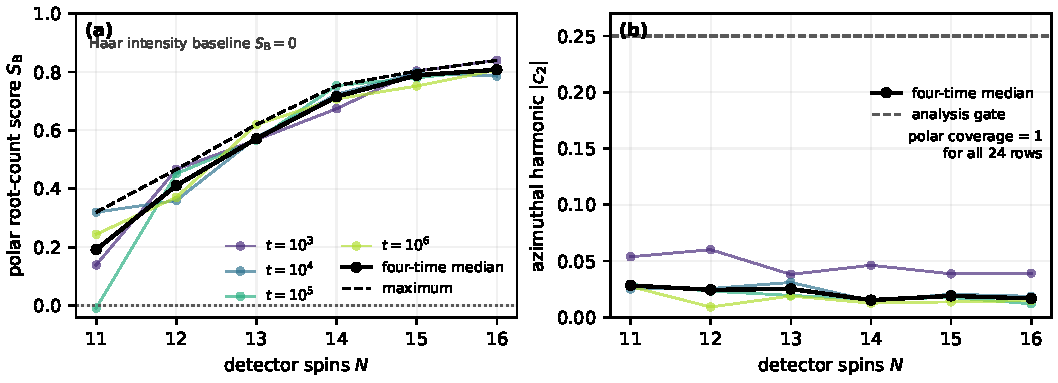
\includegraphics[width=0.91\textwidth]{matched_field_scaling.pdf}
\caption{\textbf{Structure versus the Haar null.}  (a) The four stored times, their median, and maximum.  The median polar score rises monotonically from $0.192$ at $N=11$ to $0.807$ at $N=16$; the dotted line is the intensity-level Haar baseline, not a finite-$d$ sample mean.  (b) The azimuthal second harmonic remains below the analysis gate, and polar coverage is unity for all rows.  Lines guide the eye.  The times are deterministic samples, so no stochastic error bars or thermodynamic extrapolation are implied.}
\label{fig:scaling}
\end{figure*}

The trend in Fig.~\ref{fig:scaling} contrasts this structured ring with the Haar one-point-intensity baseline, but does not provide a finite-$d$ Haar null distribution or identify a universal Hamiltonian class.  Broader post-cutoff controls show that heavy radial tails, coverage, and low azimuthal anisotropy are separate requirements; high polar scores can occur in nearly meridional clouds (Supplement).  We therefore make no chaos, integrability, or many-body-localization claim.

\emph{Interpretation.}---Three questions must remain separate.  \emph{Existence} is answered exactly: pole-compatible product boundary states are projective pencil roots with antipodal outcome labels.  \emph{Statistics} receives a sharp null theorem and one controlled geometric trend: Haar roots are isotropic, whereas a matched many-body ring develops a nearly dipolar full-sphere asymmetry.  \emph{Selection} is open: algebraic multiplicity is not a physical probability measure, different roots generally require different detector microstates, and instantaneous factorization does not demonstrate stable, distinguishable, redundant records.

Thus the most serious objection is also the cleanest boundary of the result: the work constructs and classifies measurement-compatible states but does not explain why nature occupies them.  What it establishes is a concrete many-body classification problem---which unitary Hamiltonians generate an outcome-root geometry, preparation measure, and record structure compatible with measurement?  Generic scrambling is not enough; the quantum arrow of measurement, if unitary, must be written in the detector's structure.

\begin{acknowledgments}
Author, affiliation, funding, and contribution information must be supplied before submission.
\end{acknowledgments}

\section*{Data availability}
The manuscript figures, post-processing script, hashes, provenance registry, and source paths are included in the accompanying package.  The large raw arrays are presently stored in local, Git-ignored campaign directories identified in the Supplemental Material; they must be deposited in a persistent archive before submission.

\bibliography{references}
\end{document}
